%%%%%%%%%%%%%%%%%%%%%%%%%%%%%%%%%%%%%%%%%
% Programming/Coding Assignment
% LaTeX Template
%
% This template has been downloaded from:
% http://www.latextemplates.com
%
% Original author:
% Ted Pavlic (http://www.tedpavlic.com)
%
% Note:
% The \lipsum[#] commands throughout this template generate dummy text
% to fill the template out. These commands should all be removed when 
% writing assignment content.
%
% This template uses a Perl script as an example snippet of code, most other
% languages are also usable. Configure them in the "CODE INCLUSION 
% CONFIGURATION" section.
%
%%%%%%%%%%%%%%%%%%%%%%%%%%%%%%%%%%%%%%%%%

%----------------------------------------------------------------------------------------
%	PACKAGES AND OTHER DOCUMENT CONFIGURATIONS
%----------------------------------------------------------------------------------------

\documentclass{article}

\usepackage{fancyhdr} % Required for custom headers
\usepackage{lastpage} % Required to determine the last page for the footer
\usepackage{extramarks} % Required for headers and footers
\usepackage[usenames,dvipsnames]{color} % Required for custom colors
\usepackage{graphicx} % Required to insert images
\usepackage{listings} % Required for insertion of code
\usepackage{courier} % Required for the courier font
\usepackage{lipsum} % Used for inserting dummy 'Lorem ipsum' text into the template
\usepackage{setspace}
\usepackage{color}
\usepackage{comment}
\usepackage{caption}

\usepackage{hyperref}
\usepackage{natbib}
\usepackage{underscore}
\usepackage{subfigure}
\usepackage{fixltx2e}

\hypersetup{
    colorlinks=true,
    linkcolor=blue,
    filecolor=magenta,      
    urlcolor=cyan,
    breaklinks=true
}

%\usepackage[]{algorithm2e}
\usepackage{pdfpages}




%For python inclusion (http://widerin.org/blog/syntax-highlighting-for-python-scripts-in-latex-documents)
\definecolor{Code}{rgb}{0,0,0}
\definecolor{Decorators}{rgb}{0.5,0.5,0.5}
\definecolor{Numbers}{rgb}{0.5,0,0}
\definecolor{MatchingBrackets}{rgb}{0.25,0.5,0.5}
\definecolor{Keywords}{rgb}{0,0,1}
\definecolor{self}{rgb}{0,0,0}
\definecolor{Strings}{rgb}{0,0.63,0}
\definecolor{Comments}{rgb}{0,0.63,1}
\definecolor{Backquotes}{rgb}{0,0,0}
\definecolor{Classname}{rgb}{0,0,0}
\definecolor{FunctionName}{rgb}{0,0,0}
\definecolor{Operators}{rgb}{0,0,0}
\definecolor{Background}{rgb}{0.98,0.98,0.98}

% Margins
\topmargin=-0.45in
\evensidemargin=0in
\oddsidemargin=0in
\textwidth=6.5in
\textheight=9.0in
\headsep=0.25in

\linespread{1.1} % Line spacing

% Set up the header and footer
\pagestyle{fancy}
\lhead{\hmwkAuthorName} % Top left header
%\chead{\hmwkClass\ (\hmwkClassInstructor\ \hmwkClassTime): \hmwkTitle} % Top center head
\chead{\hmwkClass\ (\hmwkClassInstructor): \hmwkTitle} % Top center head
\rhead{\firstxmark} % Top right header
\lfoot{\lastxmark} % Bottom left footer
\cfoot{} % Bottom center footer
\rfoot{Page\ \thepage\ of\ \protect\pageref{LastPage}} % Bottom right footer
\renewcommand\headrulewidth{0.4pt} % Size of the header rule
\renewcommand\footrulewidth{0.4pt} % Size of the footer rule

\setlength\parindent{0pt} % Removes all indentation from paragraphs

%----------------------------------------------------------------------------------------
%	CODE INCLUSION CONFIGURATION
%----------------------------------------------------------------------------------------

\definecolor{MyDarkGreen}{rgb}{0.0,0.4,0.0} % This is the color used for comments
\lstloadlanguages{Perl} % Load Perl syntax for listings, for a list of other languages supported see: ftp://ftp.tex.ac.uk/tex-archive/macros/latex/contrib/listings/listings.pdf
\lstset{language=Perl, % Use Perl in this example
        frame=single, % Single frame around code
        basicstyle=\small\ttfamily, % Use small true type font
        keywordstyle=[1]\color{Blue}\bf, % Perl functions bold and blue
        keywordstyle=[2]\color{Purple}, % Perl function arguments purple
        keywordstyle=[3]\color{Blue}\underbar, % Custom functions underlined and blue
        identifierstyle=, % Nothing special about identifiers                                         
        commentstyle=\usefont{T1}{pcr}{m}{sl}\color{MyDarkGreen}\small, % Comments small dark green courier font
        stringstyle=\color{Purple}, % Strings are purple
        showstringspaces=false, % Don't put marks in string spaces
        tabsize=5, % 5 spaces per tab
        %
        % Put standard Perl functions not included in the default language here
        morekeywords={rand},
        %
        % Put Perl function parameters here
        morekeywords=[2]{on, off, interp},
        %
        % Put user defined functions here
        morekeywords=[3]{test},
       	%
        morecomment=[l][\color{Blue}]{...}, % Line continuation (...) like blue comment
        numbers=left, % Line numbers on left
        firstnumber=1, % Line numbers start with line 1
        numberstyle=\tiny\color{Blue}, % Line numbers are blue and small
        stepnumber=5 % Line numbers go in steps of 5
}

% Creates a new command to include a perl script, the first parameter is the filename of the script (without .pl), the second parameter is the caption
\newcommand{\perlscript}[2]{
\begin{itemize}
\item[]\lstinputlisting[caption=#2,label=#1]{#1.pl}
\end{itemize}
}


%----------------------------------------------------------------------------------------
%	DOCUMENT STRUCTURE COMMANDS
%	Skip this unless you know what you're doing
%----------------------------------------------------------------------------------------

% Header and footer for when a page split occurs within a problem environment
\newcommand{\enterProblemHeader}[1]{
\nobreak\extramarks{#1}{#1 continued on next page\ldots}\nobreak
\nobreak\extramarks{#1 (continued)}{#1 continued on next page\ldots}\nobreak
}

% Header and footer for when a page split occurs between problem environments
\newcommand{\exitProblemHeader}[1]{
\nobreak\extramarks{#1 (continued)}{#1 continued on next page\ldots}\nobreak
\nobreak\extramarks{#1}{}\nobreak
}

\setcounter{secnumdepth}{0} % Removes default section numbers
\newcounter{homeworkProblemCounter} % Creates a counter to keep track of the number of problems

\newcommand{\homeworkProblemName}{}
\newenvironment{homeworkProblem}[1][Problem \arabic{homeworkProblemCounter}]{ % Makes a new environment called homeworkProblem which takes 1 argument (custom name) but the default is "Problem #"
\stepcounter{homeworkProblemCounter} % Increase counter for number of problems
\renewcommand{\homeworkProblemName}{#1} % Assign \homeworkProblemName the name of the problem
\section{\homeworkProblemName} % Make a section in the document with the custom problem count
\enterProblemHeader{\homeworkProblemName} % Header and footer within the environment
}{
\exitProblemHeader{\homeworkProblemName} % Header and footer after the environment
}

\newcommand{\problemAnswer}[1]{ % Defines the problem answer command with the content as the only argument
\noindent\framebox[\columnwidth][c]{\begin{minipage}{0.98\columnwidth}#1\end{minipage}} % Makes the box around the problem answer and puts the content inside
}

\newcommand{\homeworkSectionName}{}
\newenvironment{homeworkSection}[1]{ % New environment for sections within homework problems, takes 1 argument - the name of the section
\renewcommand{\homeworkSectionName}{#1} % Assign \homeworkSectionName to the name of the section from the environment argument
\subsection{\homeworkSectionName} % Make a subsection with the custom name of the subsection
\enterProblemHeader{\homeworkProblemName\ [\homeworkSectionName]} % Header and footer within the environment
}{
\enterProblemHeader{\homeworkProblemName} % Header and footer after the environment
}

%----------------------------------------------------------------------------------------
%	NAME AND CLASS SECTION
%----------------------------------------------------------------------------------------
%#MOD
\newcommand{\hmwkTitle}{Assignment\ \#4 } % Assignment title
%\newcommand{\hmwkDueDate}{Monday,\ January\ 1,\ 2012} % Due date
\newcommand{\hmwkClass}{Web Science} % Course/class
%\newcommand{\hmwkClassTime}{10:30am} % Class/lecture time
\newcommand{\hmwkClassInstructor}{Alexander Nwala} % Teacher/lecturer
\newcommand{\hmwkAuthorName}{Mohd. Nauman Siddique} % Your name

%----------------------------------------------------------------------------------------
%	TITLE PAGE
%----------------------------------------------------------------------------------------

\title{
\vspace{2in}
\textmd{\textbf{\hmwkClass:\ \hmwkTitle}}\\
%\normalsize\vspace{0.1in}\small{Due\ on\ \hmwkDueDate}\\
%\vspace{0.1in}\large{\textit{\hmwkClassInstructor\ \hmwkClassTime}}
\vspace{0.1in}\large{\textit{\hmwkClassInstructor}}
\vspace{3in}
}

\author{\textbf{\hmwkAuthorName}}
%#MOD
\date{Saturday, March 16, 2019} % Insert date here if you want it to appear below your name

%----------------------------------------------------------------------------------------

\begin{document}

\maketitle



%----------------------------------------------------------------------------------------
%	TABLE OF CONTENTS
%----------------------------------------------------------------------------------------

%\setcounter{tocdepth}{1} % Uncomment this line if you don't want subsections listed in the ToC

\newpage
\tableofcontents
\newpage

%----------------------------------------------------------------------------------------
%	PROBLEM 1
%----------------------------------------------------------------------------------------

% To have just one problem per page, simply put a \clearpage after each problem

\begin{homeworkProblem}
 Determine if the friendship paradox holds for my Facebook
account.* Compute the mean, standard deviation, and median of the
number of friends that my friends have.  Create a graph of the
number of friends (y-axis) and the friends (x-axis) themselves, sorted by
number of friends (y-axis).  (The friends don't need to be labeled
on the x-axis: just f1, f2, f3, ... fn.)  Do include me in the graph
and label me accordingly.

* = This used to be more interesting when you could more easily download
your friend's friends data from Facebook.  Facebook now requires each
friend to approve this operation, effectively making it impossible.

I will upload a csv file of my 2014 friends list on the \#assignment-4 slack channel

%\problemAnswer
%{
    \begin{verbatim}\end{verbatim}
    \textbf{SOLUTION}\\

The solution to the problem is as below:
\begin{enumerate}
 \item \textbf{Friend List }: The csv file for facebook friend list uploaded on slack has 99 entries. But the problem mentioned \emph{acnwala} has 2014 friends. I have used 2014 as the friend count for \emph{acnwala} in my graph.

\item \textbf{Graph}: Figure \ref{facebook} shows the friendship paradox for acnwala's Facebook account.  The mode value is 266, mean value is 542 and standard deviation is 539. The number of friends following for acnwala is 2014. As, the mean and standard deviation values are very cloe, they appear as a single point in my graph.

\item \textbf{Friendship Paradox}: It does not hold as the mean list of friends is less than acnwala's friend list count. 
\begin{figure}[ht]
  \centering
  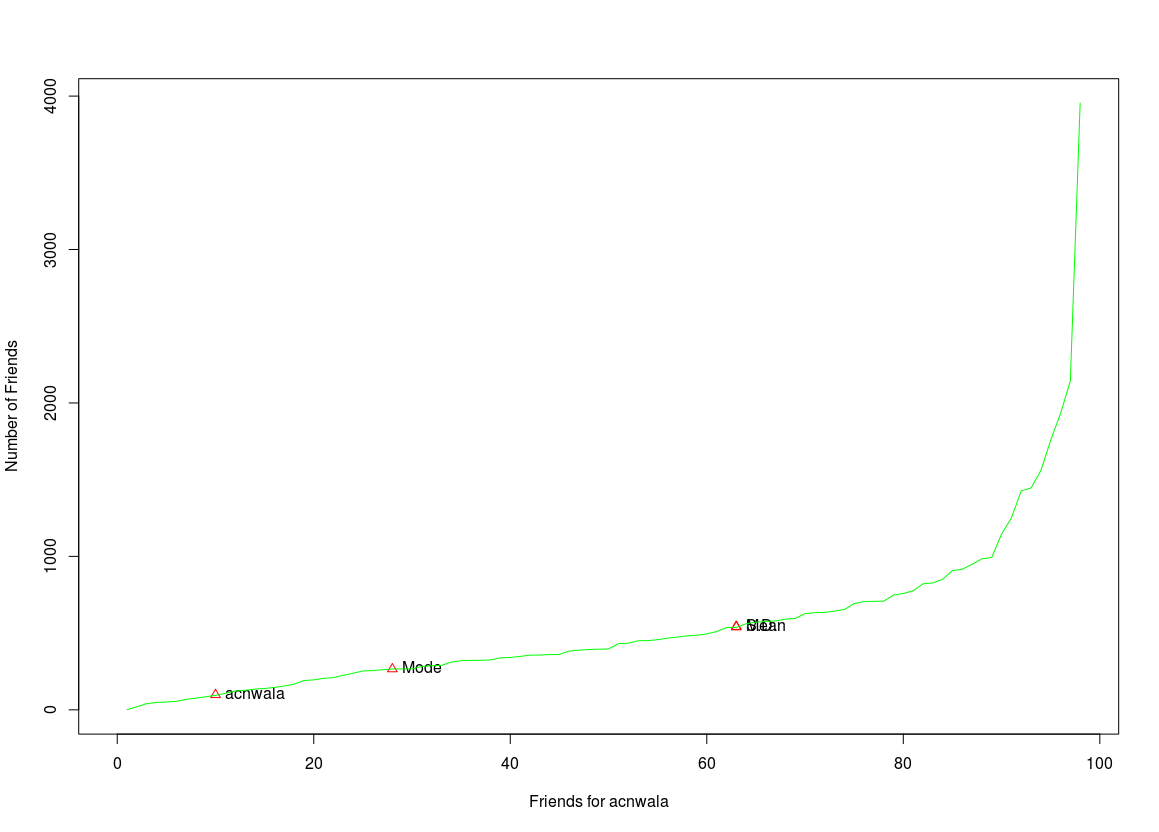
\includegraphics[width=0.9\textwidth]{facebook.png}
  \caption{Friendship Paradox for friendship of acnwala's Facebook account}
  \label{facebook}
\end{figure}
\end{enumerate}
  
%}

\end{homeworkProblem}

%----------------------------------------------------------------------------------------
%   PROBLEM 2
%----------------------------------------------------------------------------------------

\begin{homeworkProblem}

Determine if the friendship paradox holds for your Twitter account.
Since Twitter is a directed graph, use "followers" as value you measure
(i.e., "do your followers have more followers than you?").

Generate the same graph as in question \#1, and calcuate the same 
mean, standard deviation, and median values.

For the Twitter 1.1 API to help gather this data, see:

\url{https://developer.twitter.com/en/docs/accounts-and-users/follow-search-get-users/api-reference/get-followers-list}

If you do not have followers on Twitter (or don't have more than 50),
then use my twitter account "acnwala".


%\problemAnswer
%{
    \begin{verbatim}\end{verbatim}
    \textbf{SOLUTION}\\

The solution to the problem is as below:
\begin{enumerate}
 \item \textbf{Fetch Follower List }: I have fetched follower's list from Twiter API for \emph{phonedude_mln}. Some of the followers had very large following list, so I have used log base 2 in my graphs to plot it.
\item \textbf{Graph}: Figure \ref{Followers} shows the friendship paradox for phonedude_mln's Twitter account for followers. The mode value is 0, mean value is 273 and standard deviation is 8. The number of Twitter followers for phonedude_mln is 925. 

\item \textbf{Friendship Paradox}: It does not hold as the mean list of followers is less than phonedude_mln's follower list count.
\begin{lstlisting}[language=python, breaklines=true]
'''
Function to fetch Twitter followers list 
'''


def fetch_twitter_followers():
    api = create_twitter_instance()
    file_object = open("TwitterData.csv","w")
    fieldnames = ["Name", "Followers", "Friends"]
    writer = csv.DictWriter(file_object, fieldnames=fieldnames)
    writer.writeheader()
    response = api.GetFollowers(screen_name="phonedude_mln")
    for friend in response:

        insert_row = {"Name": friend.name, "Followers": math.log(friend.followers_count + 1, 2),
                      "Friends": math.log(friend.friends_count + 1, 2)}
        writer.writerow(insert_row)
    file_object.close()
\end{lstlisting}
\begin{figure}[ht]
  \centering
  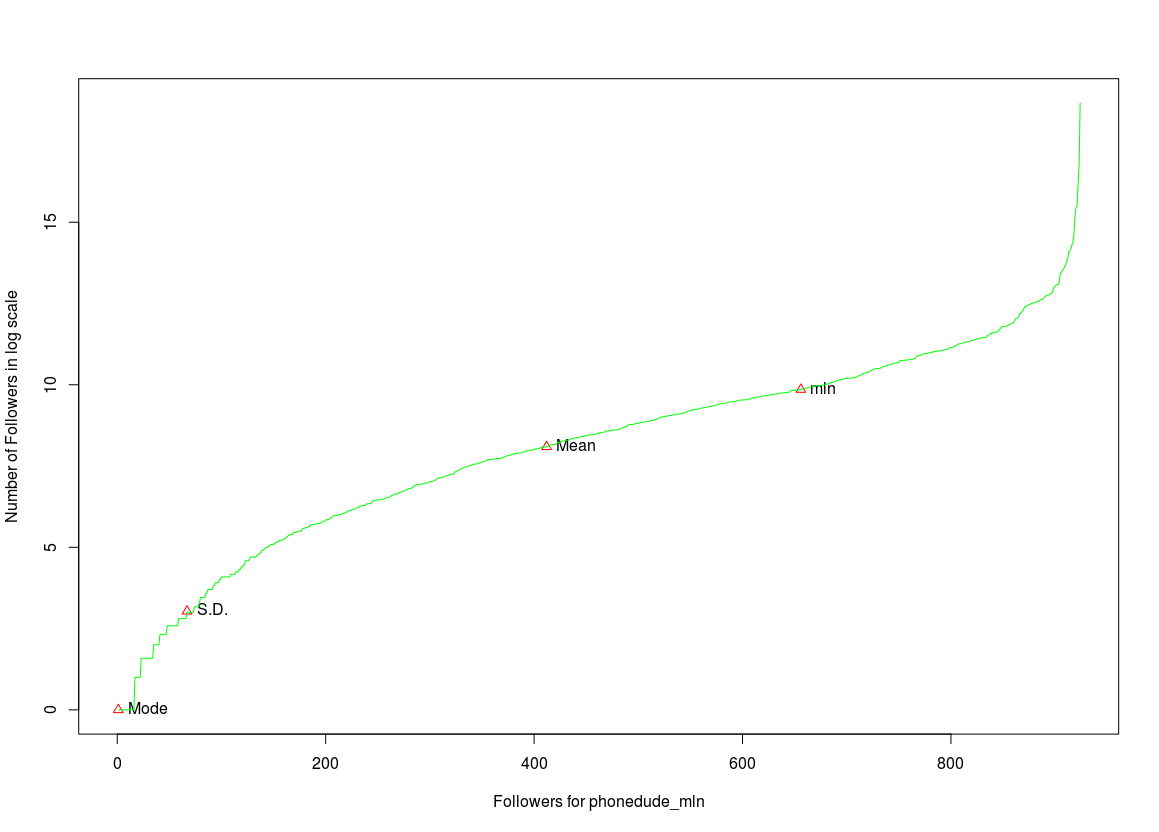
\includegraphics[width=0.9\textwidth]{Followers.png}
  \caption{Friendship Paradox for followers of phonedude_mln's Twitter account}
  \label{Followers}
\end{figure}
\end{enumerate}
   %}

\end{homeworkProblem}

%----------------------------------------------------------------------------------------
%   PROBLEM 3
%----------------------------------------------------------------------------------------

\begin{homeworkProblem}

Repeat question \#2, but change "followers" to "following"?  In
other words, are the people I am following following more people?

For the Twitter 1.1 API to help gather this data, see:

\url{https://developer.twitter.com/en/docs/accounts-and-users/follow-search-get-users/api-reference/get-friends-list}

%\problemAnswer
%{
    \begin{verbatim}\end{verbatim}
    \textbf{SOLUTION}\\
The solution to the problem is as below:
\begin{enumerate}
 \item \textbf{Fetch Follower List }: I have fetched following's list from Twiter API for \emph{phonedude_mln}. Some of the following had very large following list, so I have used log base 2 in my graphs to plot it.
\item \textbf{Graph}:Figure \ref{Following} shows the friendship paradox for phonedude_mln's Twitter account for following. The mode value is 1, mean value is 245 and standard deviation is 6. The number of Twitter following for phonedude_mln is 450. 

\item \textbf{Friendship Paradox}: It does not hold as the mean list of following is less than phonedude_mln's following list count.
\begin{lstlisting}[language=python, breaklines=true]
'''
Function to fetch Twitter following list 
'''


def fetch_twitter_following():
    api = create_twitter_instance()
    file_object = open("TwitterDataFollowing.csv","w")
    fieldnames = ["Name", "Followers", "Friends"]
    writer = csv.DictWriter(file_object, fieldnames=fieldnames)
    writer.writeheader()
    response = api.GetFriends(screen_name="phonedude_mln")
    for friend in response:

        insert_row = {"Name": friend.name, "Followers": math.log(friend.followers_count + 1, 2),
                      "Friends": math.log(friend.friends_count + 1, 2)}
        writer.writerow(insert_row)
    file_object.close()
\end{lstlisting}
\begin{figure}[ht]
  \centering
  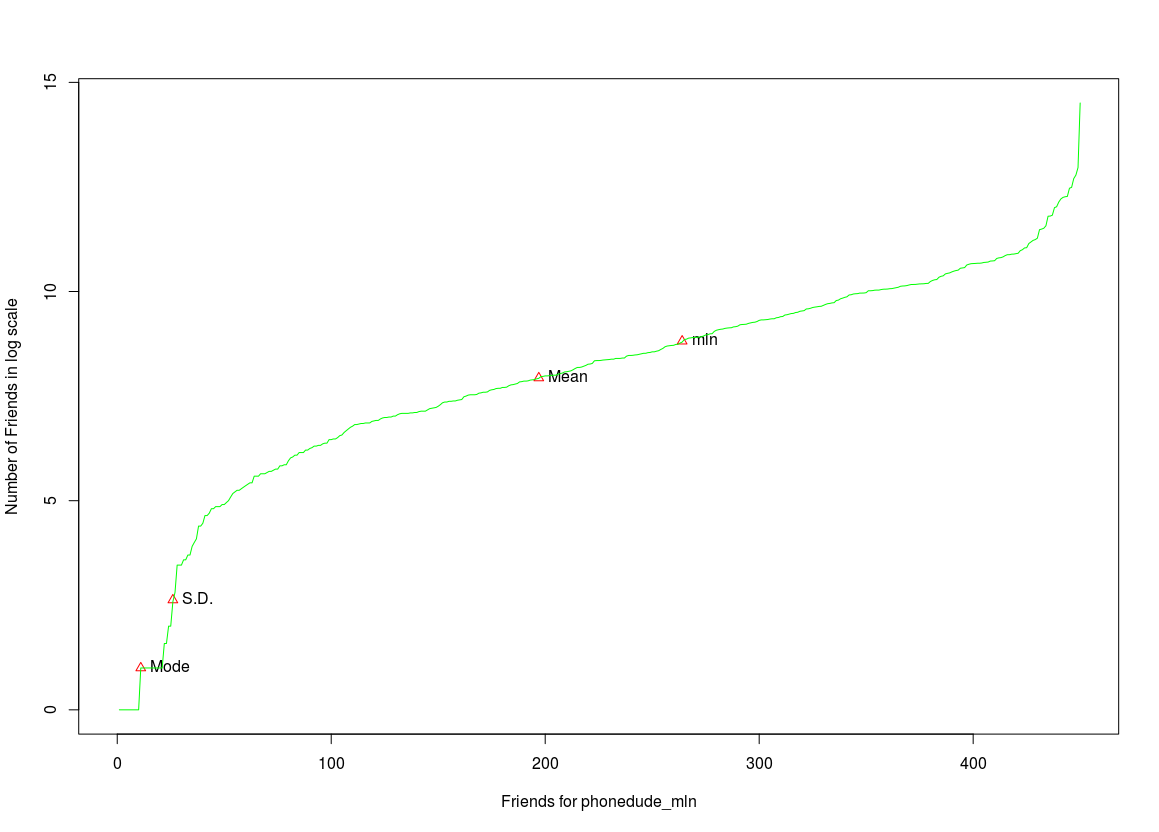
\includegraphics[width=0.9\textwidth]{Following.png}
  \caption{Friendship Paradox for following of phonedude_mln's Twitter account}
  \label{Following}
\end{figure}
\end{enumerate}
\end{homeworkProblem}


\end{document}
    


   

    

    

    
   
